\section{Field-Programmable Gate Arrays}
\label{bg:sec:fpga}

\subsection{Computing Architectures}
\label{bg:sub:computing_architectures}

When it comes to implementing computations, we often choose from a
spectrum of computing machines.  These choices range from ones with fixed
architectures that computes by executing \emph{software} designs, such as
CPUs and general-purpose graphics processing units (GPUs), to ones that can
implement custom \emph{hardware} architectures, such as FPGAs and ASICs
(application-specific integrated circuits).

There has been a great amount of efforts in recent decades to make
fixed-architecture machines run as fast as possible; many novel and intricate
ideas were proposed and we now have many general circuitries in CPUs to
improve their performance~\cite{comparch}.  For instance, CPUs could have a
pipeline that spans several clock cycles to fetch and decode instructions,
access data from memory or registers to carry out computations.  At the same
time, they would make predictions about the branches taken in control-flows,
as the pipeline must be flushed if an incorrect instruction is fetched,
incurring a penalty in speed.  They could also exploit instruction-level,
data-level and thread-level parallelism, in order to maximize opportunities to
parallelize computations.  These are just the tip of the iceberg, as many other
architectural advancements exist.

The great majority of fixed-architecture computing machines are based on
\emph{von Neumann architecture}, which consists of three parts: a computation
unit, a memory and a bus between them to move data back and forth.  Often
applications running on these machines could spend a majority of their time
and energy to move data and instructions in the memory from/to the right
location in the processor as fast as possible, in order to carry out arithmetic
computations.  Because computational tasks frequently reuse input data and
intermediate results, a hierarchy of caches, in tandem with cache-aware
compiler optimizations~\cite{kowarschik03}, are often used to mitigate the
costs of exchanging data between the processor and the memory.  Despite
these optimization efforts to run software code as fast as possible, the
processor-memory bus, which is often referred to as the \emph{von Neumann
bottleneck}~\cite{backus78}, inherently exist and it remains the limiting
factor of performance in the architecture, and this phenomenon is known to many
as \emph{hitting the memory wall}~\cite{bacon13, wulf94}.

Custom architectures in general achieve much higher performance, thanks to
their ability to implement arbitrary digital circuits specifically designed for
the application under consideration, and spatially distribute memory bandwidth
and computations.  This is in stark contrast to microprocessors such as CPUs
and GPUs, which utilize general-purpose circuitry to cope with a wide-range
of applications.  ASICs provide the best power efficiency and performance
among all above architectures, however they are often associated with long
development cycles and high costs; any updates to the design would require a
complete and expensive re-spinning of the circuits~\cite{bacon13}, as they
are inherently non-programmable.  FPGAs provide the best trade-off between
processors and ASICs.  Not only do FPGAs have better performance and power
characteristics than fixed architectures, they also offer high programmability
which makes FPGAs cost-effective low-volume ASIC replacements~\cite{karen04,
bacon13}.  At the same time, with a much shorter development period than ASICs,
hardware designs on FPGAs can be implemented with a much lower cost, and
shorter time to market enables a substantially larger profit by a competitively
early market entry~\cite{semico12}.  For the above reasons, being able to
expose parallelism from bit-level all the way to the loop and task level, FPGAs
have been increasingly used as high-performance and low-power alternatives to
CPUs and GPUs for many classes of applications~\cite{bacon13, brodtkorb10,
sirowy08}.  For example, Thomas~\etal~\cite{thomas09} reported a FPGA-based
random number generator can obtain a $260\times$ speed-up, while costing less
than 1\% of energy to produce each random sample when compared to its software
counterpart running on a CPU\@.  Microsoft embedded Stratix V FPGAs in their
data center, reducing the latency of their Bing web search engine by a factor
of 95\%~\cite{catapult}.


\subsection{FPGA Architecture}
\label{bg:sub:fpga_architecture}

FPGAs owe their high performance and power efficiency to the design of the
architecture, we thus use Altera Stratix V~\cite{stratix5} as an example to
explain the architecture.  Stratix V fabric contain of an two-dimensional array
of logic array blocks (LABs).  Each LAB consists of an array of 10 adaptive
logic modules (ALMs); Figure~\ref{bg:fig:alm} shows a high-level block diagram
of an ALM in Stratix V.  In an ALM, multiplexers can be configured to choose
whether full adders and registers are used.  Dedicated full adders enable more
complex boolean functions to be implemented in a single ALM, whereas the use of
registers, which store intermediate values, determines whether the circuit is
combinational or sequential.  The two look-up tables (LUTs) in an ALM can be
configured to compute a combination of two arbitrary boolean functions, each
with up to 5 inputs from 8 inputs in total.  Stratix 10, slated to be released
in the next couple of years, has up to 1.87 million ALMs and 7.47 registers in
total for the most demanding applications~\cite{stratix10stat}.  Interconnects,
another class of key configurable resources on FPGAs, enable the inputs and
outputs of ALMs to be wired, in order to form larger and complete circuits from
the two-dimensional array of ALMs.  This allows the FPGA fabric to realize
arbitrary digital circuits.
\begin{figure}[ht]
    \centering
    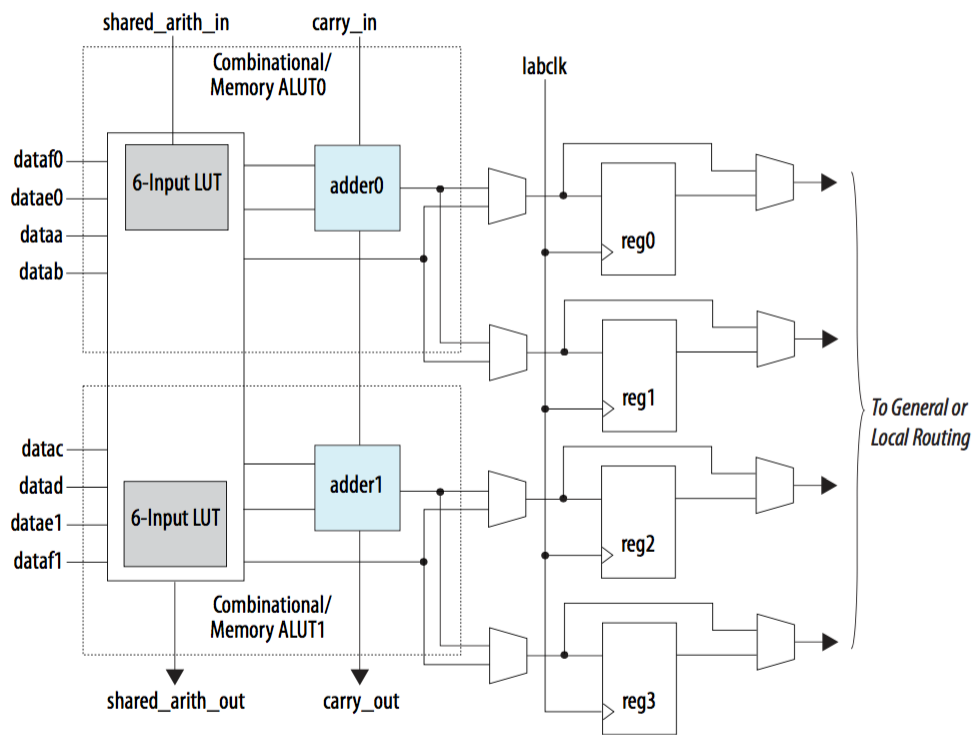
\includegraphics[width=0.8\linewidth]{bg/fig/alm.png}
    \caption{%
        A high-level block diagram of an ALM in Stratix V, from Stratix V
        Device Handbook~\cite{stratix5}.
    }\label{bg:fig:alm}
\end{figure}

% distributed memory and DSP elements

FPGAs with enough ALMs and interconnects can implement arbitrary digital
designs; this versatile architecture therefore overcomes the memory wall
problem by not restricting itself to von Neumann architecture.  As we have
mentioned earlier, FPGAs can implement a circuit that is individually tailored
for the application, in contrary, CPUs have general-purpose circuitries
that perform well across a range of applications, which may have lower
power-efficiency and performance.  Moreover, unlike the CPU which only has a
small set of registers, the FPGA with its flexibility and abundant registers,
allows designs to place memory and computation units in close proximity.

Traditionally, multipliers, when implemented in FPGAs, cost a large number of
ALMs.  Stratix devices thus further include an array of hardened components
to carry out arithmetic operations distributed on the FPGA fabric, known as
\emph{digital-signal processing} blocks (DSPs, or simply DSPs).  Because
of the dedicated hardened circuits, DSPs compute faster than arithmetic
operators formed by ALMs only, meanwhile they free ALM resources to perform
more non-arithmetic computations.  In Stratix V, each variable-precision
DSP is paired with a LAB\@.  These DSPs, can be configured in
combinations to perform a wide variety of arithmetic operations, ranging from
using a single DSP element to synthesize three multipliers with two 9-bit
inputs, up to combining four DSPs to form a complex-number multiplier
with two 27-bit inputs~\cite{stratix5}.  Computations with larger inputs can
also be implemented by using ALMs and DSPs to form larger arithmetic
circuits.  Finally, Stratix 10 will further introduce hardened floating-point
DSPs, enabling IEEE 754~\cite{ieee754} single-precision floating-point
additions and multiplications, achieving a performance of up to 10 tera
floating-point operations per second (TFLOPS)~\cite{stratix10fp}.  These DSP
blocks can also be adapted to multiply fixed-point inputs.

DSPs accelerate arithmetic computations, however they need to be supplied
with inputs as fast as they can process to fully utilize them.  Fortunately
in general, in most applications, data are frequently reused by the same
computation unit.  Stratix V therefore include dedicated embedded memory called
M20K blocks (20 Kb storage) that can be arranged and combined into dual-port
RAMs.  Half of the LABs on the device, called MLABs can also be configured to
become a 640-bit RAMs.  These memory blocks are distributed across the FPGA
fabric, so that DSPs can find them in proximity.


\subsection{RTL Design Flow}
\label{bg:sub:rtl_design}

Modern FPGAs---with up to several million LUTs, and thousands of
embedded memory and DSP blocks, wired through a programmable fabric of
interconnects---are humanly intractable to program at the granularity of these
individual components~\cite{kapre08}.  FPGA applications therefore are commonly
written in register-transfer level (RTL) hardware descriptions languages (HDL),
such as Verilog~\cite{verilog} and VHDL~\cite{vhdl}.  These HDL source programs
implements the desired hardware by describing logics between registers.
Electronic design automation (EDA) tools can then automatically translate these
descriptions into hardware circuits in FPGAs.

EDA tools, go through several stages to synthesize HDL source code
into circuits, To explain these stages in depth, we take Altera
Quartus II~\cite{quartus} as an example, which design flow is shown in
Figure~\ref{fig:quartus}.
\begin{figure}[ht]
    \centering
    \includegraphics[width=\textwidth]{bg/fig/quartus}
    \caption{Quartus II design flow from~\cite{quartus}.}\label{fig:quartus}
\end{figure}

Quartus II starts its compilation of the source code by verifying source code
for syntax and semantic errors and design specification for inconsistencies,
then apply a methodology, called \emph{technology mapping}, which maps
a network of device-independent logic gates in logic expressions onto a
network of functional blocks (such as LUTs, DSPs and memory blocks) in
the target FPGA device~\cite{cong08}; this generated network is known as
a \emph{technology-mapped netlist}.  In this process, synthesis tools may
optimize the circuit by performing additional transformations such as redundant
logic removal~\cite{quartus}.  The following stage, place \& route, utilizes a
heuristic placement algorithm, which takes as it inputs the netlist, together
with a device map showing the location of each of its functional units, in
order to select a legal location on the FPGA for each functional block in the
netlist, such that the routing of these blocks is optimized~\cite{betz08}.
In general, synthesis tools allow some freedom in the user's preference of
the placement of circuit.  Additional automated optimizations can be applied
to improve performance.  For example, Quartus II has the option to enable
\emph{register retiming}~\cite{quartus}, which allows registers to move across
combinational logic to reduce critical path delay, \ie~the longest delay
required for an output of any source register to propagate to the input of
any target register in the circuit.  The end result of this step is a circuit
schematic on the target FPGA\@; in the next step, the tool thus computes
the longest delay of all critical paths, which determines the frequency at
which the application can run.  Users can also inspect the list of critical
paths and their delay statistics, so that one can focus their effort on
optimizing the timing of them by, for instance, adding registers in critical
paths.  The user can then choose to simulate the design using EDA simulation
tools.  Finally, the circuit generated by the tool can be translated into a
\emph{bitstream}, which is binary data that can be used to program the FPGA\@.
Similar to processors, which can be programmed by incrementally reading and
executing instructions from an executable program file, a bitstream is used
to program the individual components such as LUTs, DSP blocks, dedicated
memory blocks and interconnects on an FPGA, so the circuit can be formed on
the device.  The difference between them is that while processors continuously
read instructions from memory, FPGAs are typically programed only once during
the initial setup, and the bitstream data are used spatially rather than
sequentially~\cite{guccione08}.
